\question \textbf{Probabilities of accepted mutations}

Use a phylogenetic tree below to calculate the probabilities of accepted mutations. The tree contains sequences of four OTUs.

\begin{figure}[H]
      \centering
      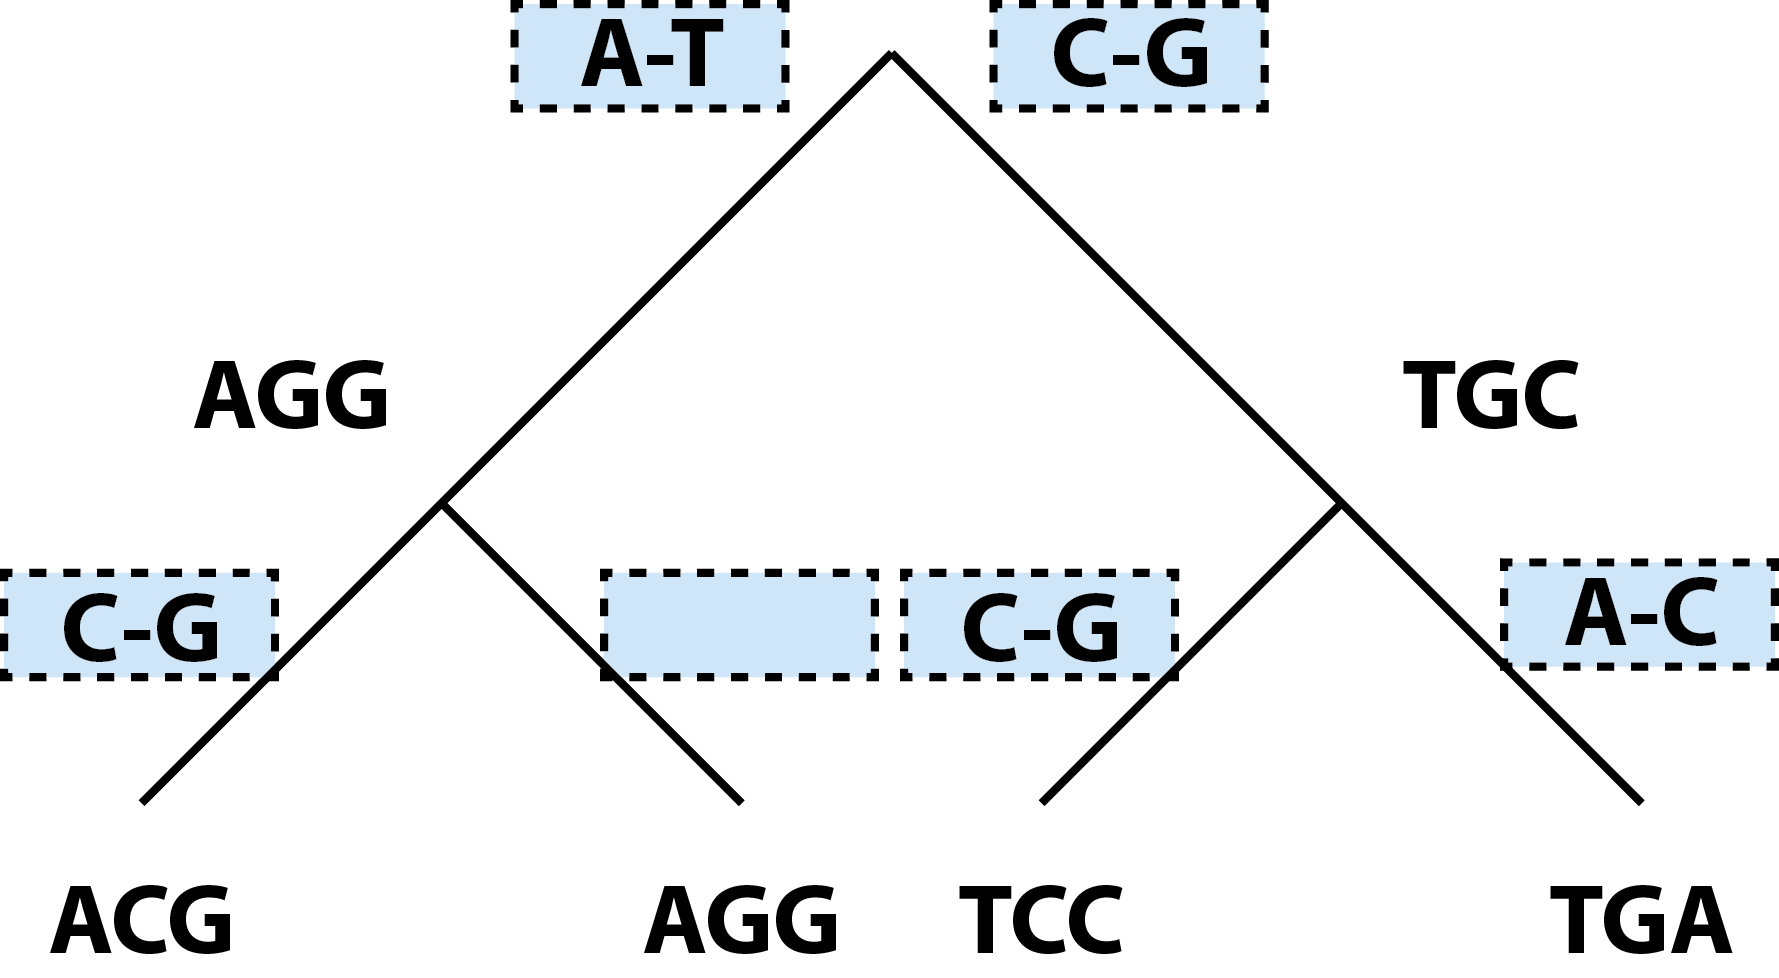
\includegraphics[width=0.4 \textwidth]{fig11/tree_sol.png}
\end{figure}

\begin{parts}

\vspace{0.1 in}

%% (a)
  \part Estimate the mutations and fill them in the boxes next to the edges.
  
  \bigskip 

%% (b)
  \part Count the occurrences of mutations and fill them in the matrix. Note that a mutation A $\rightarrow$ B is equivalent with a mutation B $\rightarrow$ A.

\begin{table}[H]
\centering
\begin{tabular}{|c|c|c|c|c|}
\hline
  & A                        & G                        & C                        & T                        \\ \hline
A &     &     &   \cellcolor[HTML]{CCE5FF} 1   & \cellcolor[HTML]{CCE5FF} 1 \\ \hline
G &     &     & \cellcolor[HTML]{CCE5FF} 3 &                          \\ \hline
C &  \cellcolor[HTML]{CCE5FF} 1 & \cellcolor[HTML]{CCE5FF} 3 &                          &                          \\ \hline
T &  \cellcolor[HTML]{CCE5FF}  1 &                          &                          &                          \\ \hline
\end{tabular}
\end{table}

%% (c)
  \part Use the following definitions and calculate $f_{CG}$, $f_C$ and $f$.
\begin{align*}
f_{ab} &: \text{The number of mutations from } a \text{ to } b \text{ or from } b\text{ to } a \\
f_a &: \text{Total number of mutations in which } a \text{ takes part} \\
f &: \text{Twice the total number of mutations} \\ \\
f_{CG} &: \colorbox{SolutionColor}{3} \\
f_C &: \colorbox{SolutionColor}{1 + 3 = 4} \\
f &: \colorbox{SolutionColor}{2 (1 + 1 + 3) = 10} \\
\end{align*}

%% (d)
  \part 	Use the following definition and calculate $p_C$.
\begin{align*}
p_a &: \text{The relative occurrence of } a \text{ in the observed sequences} \\ \\
p_C &: \colorbox{SolutionColor}{3/12} 
\end{align*}

\end{parts}

